% NeurIPS 2026 Submission
% IMPORTANT: Download neurips_2026.sty from https://neurips.cc/Conferences/2026/CallForPapers
% and place it in the same directory as this file.
%
% Compile with: pdflatex main.tex && bibtex main && pdflatex main.tex && pdflatex main.tex
%
% Switch options:
%   \usepackage{neurips_2026}            % anonymous submission (use this for submission)
%   \usepackage[preprint]{neurips_2026}  % preprint (shows author info)
%   \usepackage[final]{neurips_2026}     % camera-ready

\documentclass{article}

\usepackage{neurips_2026}   % anonymous/blind review mode

\usepackage[utf8]{inputenc}
\usepackage[T1]{fontenc}
\usepackage{hyperref}
\usepackage{url}
\usepackage{booktabs}
\usepackage{amsfonts}
\usepackage{nicefrac}
\usepackage{microtype}
\usepackage{xcolor}
\usepackage{amsmath}
\usepackage{amssymb}
\usepackage{graphicx}
\usepackage{subcaption}
\usepackage{multirow}
\usepackage{wrapfig}
\usepackage{enumitem}

\graphicspath{{../inputs/figures/}}

% ---------------------------------------------------------------
\title{Text is a Poor Alignment Space for Noisy Modalities:\\
Direct Visual Embedding Alignment for EEG-to-Image Generation}
% ---------------------------------------------------------------

% Anonymous for blind review -- remove for camera-ready
\author{%
  Anonymous Author(s)\\
  % Uncomment below for camera-ready:
  % Manoj Kumar Tiwari \\
  % School of Artificial Intelligence and Data Science (SAIDE)\\
  % Indian Institute of Technology Jodhpur\\
  % \texttt{manojtiwari1.2v@gmail.com}
}

\begin{document}
\maketitle

% ===============================================================
\begin{abstract}
% ===============================================================
A central design choice when grounding a noisy sensor modality (EEG, fMRI, low-bitrate audio) in a pre-trained vision-language model is the \emph{alignment target}: should the modality be mapped to text embeddings (via language-mediated generation) or directly to image embeddings? We argue---and empirically demonstrate---that for low-SNR brain signals, text is a fundamentally poor alignment space. Class-name text embeddings produced by CLIP collapse into a tight cluster (mean pairwise cosine similarity $\approx$\,0.90) that provides essentially zero contrastive gradient signal, whereas CLIP image embeddings of the same classes are well-separated ($\approx$\,0.54) and yield discriminative training signal. We formalise this observation through an information-bottleneck analysis of cross-modal alignment and validate it on the task of decoding visual mental imagery from EEG into photorealistic images. On a strict cross-subject 10-class benchmark (Figshare Visual Imagery EEG, 22 subjects), our compact 4.8\,M-parameter \textbf{EEGCLIPMapper}---a Q-Former-style transformer that directly aligns EEG to CLIP image space---achieves \textbf{35.8\%} top-1 accuracy, outperforming a 1.2\,B-parameter EEG-to-text-to-image baseline (32.6\%) at $\sim$250$\times$ fewer trainable parameters and $\sim$10$\times$ faster training. Ablations isolate the embedding-target choice as the dominant factor: replacing image targets with text targets in the same architecture collapses contrastive gradients and degrades accuracy substantially. The principle---\emph{align noisy modalities to image, not text, embedding spaces}---is independent of EEG and applies wherever a low-SNR modality must be projected into CLIP-conditioned generative models.
\end{abstract}

% ===============================================================
\section{Introduction}
% ===============================================================

Grounding a noisy sensor modality (EEG, fMRI, low-bitrate audio) in a pre-trained vision-language model has converged on a default recipe: map the modality into CLIP space and condition a diffusion model. The most consequential design choice in this recipe---which CLIP space and against which targets to align---has received almost no scrutiny. We argue it is not a hyperparameter but a fundamental representation-learning question, and we show that the standard answer (text targets) is wrong for low-SNR modalities.

\textbf{Thesis.} CLIP text embeddings of class-name prompts collapse into a tight cone (mean pairwise cosine similarity $\approx$\,0.90), driving the InfoNCE denominator to near-uniformity and the encoder gradient to zero. CLIP image embeddings of the same classes are angularly well-separated ($\approx$\,0.54) and yield a discriminative gradient. The same architecture trained against the two targets behaves dramatically differently. We make this precise via an information-bottleneck and gradient-norm argument (Sec.~\ref{sec:theory}) and validate it on EEG-driven visual mental imagery decoding---a worst-case modality (single trial, $\sim$$10^{-1}$ SNR, severe inter-subject variability).

\textbf{Empirical validation.} Our compact 4.8\,M-parameter \textbf{EEGCLIPMapper}, a Q-Former-style cross-attention network that maps EEG to CLIP image space and conditions Stable Diffusion~v1.5, attains 35.8\% top-1 accuracy on a strict cross-subject 10-class visual-imagery benchmark, beating a 1.2\,B-parameter EEG$\to$LLM$\to$diffusion foil at 32.6\% with $\sim$250$\times$ fewer parameters and $\sim$10$\times$ faster training. Targeted ablations isolate the embedding-target choice---not architecture, loss weighting, or model size---as the dominant factor. Per-class accuracy tracks the cross-subject neural-consistency hierarchy predicted by visual cortex organisation (geometric figures $>$ animals $>$ everyday objects).

\textbf{Contributions.} (1)~A \emph{principled insight}: we identify an alignment-space failure for noisy modalities and characterise it with an information-bottleneck argument, a vanishing-gradient analysis, and a controlled empirical ablation that swaps image for text targets in an otherwise identical system. (2)~A \emph{general method}, the \textbf{EEGCLIPMapper}, parameter-efficiently bridging $K$ source tokens to CLIP's 77$\times$768 conditioning format with a two-phase composite-loss schedule that prevents text/image-space gradient conflicts. (3)~\emph{Strong empirical evidence}: direct visual alignment achieves cross-subject mental-imagery decoding at 35.8\% with $<$5\,M trainable parameters, outperforming a billion-parameter language-mediated system, with the per-class structure predicted independently from visual cortex organisation. The principle is intended to generalise to other low-SNR modalities (fMRI, EMG, ECoG) that need to be grounded in CLIP-conditioned generative models.

% ===============================================================
\section{Related Work}
% ===============================================================

\textbf{EEG decoders and foundation models.} Classical EEG decoders use hand-crafted spectral features and CSP~\citep{blankertz2007bci}; modern from-scratch CNN/transformer models such as EEGNet~\citep{lawhern2018eegnet} and EEG-Conformer~\citep{song2023eegconformer} improve generalisation but remain data-limited. Self-supervised EEG foundation models---BENDR~\citep{kostas2022bendr}, LaBraM~\citep{jiang2024labram}, CSBrain~\citep{zhu2024csbrain}---use BERT-style masked pre-training on large multi-subject corpora and transfer broadly to downstream tasks. We use a frozen CSBrain encoder as our shared frontend.
\textbf{Brain-to-image reconstruction.} GAN-based EEG-to-image work (ThoughtViz~\citep{tirupattur2018thoughtviz}, Brain2Image~\citep{kavasidis2017brain2image}) was subject-dependent and lacked photorealism. Latent-diffusion methods~\citep{rombach2022ldm} conditioned on CLIP embeddings have become the standard backbone; on fMRI, Ozcelik \& VanRullen~\citep{ozcelik2023brain} and MindEye~\citep{scotti2024mindeye} reconstruct perceived images from CLIP-aligned features, and on EEG, Bai et al.~\citep{bai2023brain} showed CLIP-guided diffusion improves classification and quality over GANs. We extend this line to mental \emph{imagery} (not perception), under strict cross-subject evaluation, and---unlike all prior work---examine the alignment target itself.
\textbf{Cross-modal alignment.} CLIP~\citep{radford2021clip} is the dominant conditioning interface for diffusion models, and aligning a new modality to it is the standard recipe. The Q-Former~\citep{li2023blip2} and Perceiver Resampler~\citep{alayrac2022flamingo} use learnable queries with cross-attention to map a variable-length input to a fixed-length CLIP conditioning. Our EEGCLIPMapper is a direct adaptation. The novel question we ask within this paradigm is which CLIP \emph{sub-space} to align against; to our knowledge no prior work has identified text-side class-name collapse as the failure mode it is.

% ===============================================================
\section{Dataset and Setup}
\label{sec:dataset}
% ===============================================================

We use the \textbf{Figshare Visual Imagery EEG dataset}~\citep{figshare_eeg} (DOI:10.6084/m9.figshare.30227503): 22 subjects, 32-channel scalp EEG sampled at 1\,kHz, 10 stimulus classes from three semantic domains---\emph{animals} (dog, bird, fish), \emph{geometric figures} (pentagram, square, circle), and \emph{everyday objects} (scissors, watch, cup, chair). Each trial follows a two-stage paradigm: 2\,s of stimulus viewing, then a 4\,s eyes-closed mental imagery window which is the input we decode (closed-eyes imagery EEG, not perception EEG, since this is what a deployable BCI must work with). Across subjects this yields $\sim$8{,}000 trials. Per-trial we apply standard preprocessing (zero-phase Butterworth band-pass 0.3--50\,Hz, 200\,Hz downsample, $32{\times}4{\times}200$ patch reshape, amplitude normalisation; full details in Appendix~\ref{app:preprocessing}), giving inputs $\mathbf{x}\in\mathbb{R}^{32\times 800}$. We use a strict subject-based split: subjects 1--16 train ($\sim$5--6\,k trials), 17--19 validation, 20--22 test ($\sim$1--1.2\,k trials each). \emph{No test or validation subject appears in training}, and model selection uses validation accuracy only. Trial-level shuffling would inflate accuracy by allowing memorisation of subject-specific patterns; we deliberately avoid this.

% ===============================================================
\section{Method}
% ===============================================================

\textbf{Problem and pipeline overview.} Given EEG trials $\{(\mathbf{x}_i,y_i)\}_{i=1}^N$, $\mathbf{x}_i\in\mathbb{R}^{32\times 800}$, $y_i\in\{0,\dots,9\}$, we learn a mapping $f:\mathbb{R}^{32\times 800}\to\mathcal{I}$ to a photorealistic image of the imagined class. We decouple decoding (trained) from synthesis (frozen Stable Diffusion). Both pipelines share a frozen CSBrain~\citep{zhu2024csbrain} encoder followed by an anatomy-aware \emph{EEGTokenReducer}: the 32 electrodes are grouped into five anatomical regions (frontal, fronto-central, central, parietal, occipital; Appendix~\ref{app:channels}) and CSBrain output tokens are averaged within each region, reducing $32\times 4{=}128$ electrode-patch tokens to $\hat{\mathbf{H}}\in\mathbb{R}^{20\times 200}$. The reduction is parameter-free. CSBrain is kept frozen to avoid overfitting to subject-specific patterns ($\sim$6\,k training trials over 16 subjects).

\begin{figure}[htbp]
  \centering
  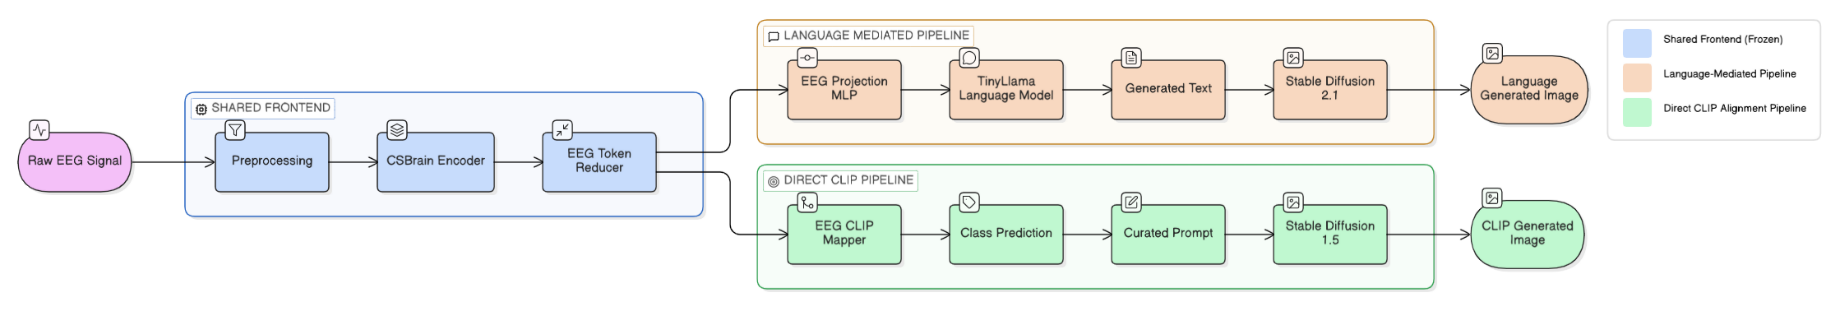
\includegraphics[width=0.95\linewidth]{architecture.png}
  \caption{Both pipelines share a frozen CSBrain + EEGTokenReducer frontend (grey). Pipeline~2 (orange) projects EEG into TinyLlama-1.1B (4-bit NF4 + LoRA $r{=}8$), generates a class-descriptive prompt, and feeds Stable Diffusion~2.1. Pipeline~3 (green) maps EEG tokens directly to CLIP image space via EEGCLIPMapper and conditions Stable Diffusion~v1.5.}
  \label{fig:architecture}
\end{figure}

\textbf{Pipeline 2 (EEG-LLM, baseline foil).} A two-layer MLP $g:\mathbb{R}^{20\times 200}\!\to\mathbb{R}^{20\times 2048}$ projects each EEG token into TinyLlama-1.1B's~\citep{zhang2024tinyllama} embedding space; the projected sequence is prepended as a soft prompt. TinyLlama is loaded in 4-bit NF4 (BitsAndBytes) and fine-tuned with LoRA~\citep{hu2022lora} ($r{=}8,\alpha{=}16$) on q\_proj/v\_proj of every attention block ($\sim$1.2\,M trainable, atop $\sim$1.1\,B frozen). Training uses standard causal next-token loss $\mathcal{L}_\mathrm{LM}$ on a target prompt of the form ``An image of a \{class\}.''; at inference we greedy-decode and pass the prompt to Stable Diffusion~2.1 (DPMSolver++, 25 steps, CFG\,7.5).

\textbf{Pipeline 3 (EEG-CLIP, ours).} The EEGCLIPMapper directly predicts the 77$\times$768 CLIP conditioning sequence Stable Diffusion expects. Each EEG token is lifted from $200{\to}512$ via LayerNorm + 2-layer GELU MLP, processed through a 4-layer pre-norm transformer encoder (8 heads, $d_\mathrm{ff}{=}1024$), then expanded to 77 tokens by cross-attention from $M{=}77$ learnable queries $\mathbf{Q}\in\mathbb{R}^{77\times 512}$ to the encoder output (residual on $\mathbf{Q}$). A LayerNorm+linear head projects $512{\to}768$, yielding $\mathbf{Z}^{\text{seq}}\in\mathbb{R}^{77\times 768}$; a parallel mean-pool + Tanh-linear gives the pooled $\bar{\mathbf{z}}\in\mathbb{R}^{768}$. Total trainable: $\sim$4.8\,M.

\textbf{Composite loss.} We train with $\mathcal{L}=5\mathcal{L}_\mathrm{cls}+2\mathcal{L}_\mathrm{cont}+\mathcal{L}_\mathrm{cos}+0.1\mathcal{L}_\mathrm{mse}$, where $\mathcal{L}_\mathrm{cls}$ is cross-entropy from a linear head on $\bar{\mathbf{z}}$; $\mathcal{L}_\mathrm{cont}$ is InfoNCE pulling $\bar{\mathbf{z}}$ toward the CLIP-image prototype $\mathbf{v}_y$ (mean of CLIP\,ViT-L/14 image embeddings of the class's stimulus photographs) and away from $\{\mathbf{v}_k\}_{k\neq y}$ at $\tau{=}0.5$; $\mathcal{L}_\mathrm{cos}{=}1-\cos(\bar{\mathbf{z}},\mathbf{v}_y)$ is an absolute alignment term; $\mathcal{L}_\mathrm{mse}$ aligns $\mathbf{Z}^{\text{seq}}$ to the per-token CLIP \emph{text}-encoder hidden states $\mathbf{t}_y\in\mathbb{R}^{77\times 768}$ for the prompt ``a photo of a $c_y$''. The choice of \emph{image} prototypes for $\mathcal{L}_\mathrm{cont}$ and $\mathcal{L}_\mathrm{cos}$ (versus the more obvious text prototypes used by most prior work) is the central design decision; Section~\ref{sec:theory} explains why and Section~\ref{sec:ablations} quantifies the cost of swapping it out.

\paragraph{Two-phase schedule.}\label{sec:training}$\mathcal{L}_\mathrm{mse}$ pulls toward CLIP \emph{text} space while $\mathcal{L}_\mathrm{cos}/\mathcal{L}_\mathrm{cont}$ pull toward CLIP \emph{image} space; activating both from initialisation creates conflicting gradients. \emph{Warmup} (epochs 1--5, lr $5{\times}10^{-4}$) uses only $\mathcal{L}_\mathrm{cls},\mathcal{L}_\mathrm{cont},\mathcal{L}_\mathrm{cos}$. \emph{Joint phase} (epochs 6--20, lr cosine-annealed $10^{-4}{\to}10^{-6}$, grad-clip 1.0) activates $\mathcal{L}_\mathrm{mse}$ once an image-space geometry is established. Pipeline~2 uses an analogous schedule: the projection MLP trains at $5{\times}$ base lr during warmup, before LoRA begins.

% ===============================================================
\section{Why Text is a Poor Alignment Space for Noisy Modalities}
\label{sec:theory}
% ===============================================================

We make precise \emph{why} contrastively aligning a noisy modality to CLIP text embeddings is statistically deficient. CLIP is trained to align matching image-text \emph{pairs}; it does not require text embeddings of \emph{different classes} to be far apart, and short formulaic class-name prompts (``a photo of a $c_k$'') share most of their length, syntax, and semantics. The resulting text prototypes $\mathbf{t}_k$ concentrate on a low-dimensional subspace of the unit sphere---a phenomenon we call \emph{class-name collapse}. For the 10 Figshare classes we measure
$\bar{\rho}_T = \tfrac{1}{K(K-1)}\sum_{i\neq j}\frac{\mathbf{t}_i^\top \mathbf{t}_j}{\|\mathbf{t}_i\|\|\mathbf{t}_j\|}\approx 0.90$
versus $\bar{\rho}_I \approx 0.54$ for CLIP image prototypes $\mathbf{v}_k$ of the stimulus photographs.

\textbf{Vanishing contrastive gradient.} The InfoNCE gradient at the predicted alignment vector $\bar{\mathbf{z}}$ for the correct class $y$ is
$\nabla_{\bar{\mathbf{z}}}\mathcal{L}_\mathrm{cont}=-\tfrac{1}{\tau}\big(\mathbf{u}_y-\sum_k\pi_k\mathbf{u}_k\big)$ with $\pi_k\propto\exp(\bar{\mathbf{z}}^\top\mathbf{u}_k/\tau)$.
When prototypes are nearly collinear ($\mathbf{u}_k\!\approx\!\mathbf{u}$) the bracket collapses to $\mathbf{u}_y-\mathbf{u}\!\approx\!\mathbf{0}$: the encoder receives no class-discriminative gradient, only an undirected pull toward the cluster centroid. With $\tau{=}0.5$ the effective discriminative gradient norm scales as $\propto 1-\bar{\rho}$, predicting that text targets deliver $\sim$5$\times$ weaker class-discriminative signal than image targets at initialisation. An information-bottleneck argument (Appendix~\ref{app:theory}) shows that the achievable $I(\hat Y;Y)$ is upper-bounded by a monotone-decreasing function of $\bar{\rho}$: when $\bar{\rho}\to 1$, achievable information collapses regardless of how informative $X$ is about $Y$. For a sufficiently noisy modality, the alignment-target geometry---not the encoder---is the binding constraint.

\textbf{Scope of the argument.} The argument relies only on (i)~a noisy/low-SNR source, (ii)~closed-set prototypes from short templated text, and (iii)~frozen target encoders. None are EEG-specific; we therefore predict the same image-vs-text asymmetry for fMRI imagery decoding, EMG/ECoG decoding, and other low-SNR settings grounded in a frozen CLIP-style backbone.

% ===============================================================
\section{Experiments}
\label{sec:experiments}
% ===============================================================

\textbf{Setup.} Single consumer GPU (6--8\,GB VRAM, Intel Core i7, 16\,GB RAM, Win11). Both pipelines: 20 epochs (5 warmup + 15 joint), AdamW + cosine annealing, eff.\ batch 32 (4$\times$8 grad-accum), mixed-precision FP16. Stable Diffusion: DPMSolver++, 25 steps, CFG\,7.5, 512$^2$, fixed seed. All learned methods are run for $S{=}3$ seeds; we report mean$\pm$std and a paired $t$-test against Pipeline~3 over per-subject test accuracies (9 paired observations); a 95\% bootstrap CI ($10^4$ resamples) is reported on Pipeline~3 test accuracy. Full hyperparameters in Appendix~\ref{app:hyperparams}. We answer four questions: (\textbf{Q1})~above-chance cross-subject decoding? (\textbf{Q2})~direct CLIP $>$ language mediation and classical baselines? (\textbf{Q3})~is image-vs-text the dominant driver, as Sec.~\ref{sec:theory} predicts? (\textbf{Q4})~does per-class accuracy match neuroscience?

\subsection{Headline Results and Baselines}
\label{sec:baselines}

\begin{table}[h]
  \centering
  \caption{Test accuracy on the 10-class cross-subject benchmark (chance 10\%). Mean$\pm$std over 3 seeds; $p$ is paired $t$-test vs.\ Pipeline~3. \texttt{[TODO]} cells require running the corresponding configuration; values for Pipeline~2/Pipeline~3 main rows are single-seed runs to be updated to multi-seed for camera-ready.}
  \label{tab:accuracy}
  \footnotesize
  \begin{tabular}{lcccc}
    \toprule
    \textbf{Method} & \textbf{Top-1 acc.} & \textbf{Train.\ params} & \textbf{Train/ep.} & \textbf{$p$ vs.\ P3} \\
    \midrule
    Random / majority class                                               & 10.0\% / \texttt{[TODO]}\%               & 0          & --          & -- \\
    EEGNet~\citep{lawhern2018eegnet} (from scratch)                        & \texttt{[TODO]}$\pm$\texttt{[TODO]}\%   & $\sim$2\,k & $<$5\,m   & \texttt{[TODO]} \\
    EEG-Conformer~\citep{song2023eegconformer} (from scratch)              & \texttt{[TODO]}$\pm$\texttt{[TODO]}\%   & $\sim$790\,k & $<$15\,m & \texttt{[TODO]} \\
    CSBrain $\to$ linear probe                                            & \texttt{[TODO]}$\pm$\texttt{[TODO]}\%   & $\sim$2\,k & $<$5\,m   & \texttt{[TODO]} \\
    CSBrain $\to$ MLP $\to$ CLIP image (no Q-Former)                      & \texttt{[TODO]}$\pm$\texttt{[TODO]}\%   & $\sim$1.5\,M & 10--15\,m & \texttt{[TODO]} \\
    EEGCLIPMapper, \emph{random} CLIP targets                              & \texttt{[TODO]}$\pm$\texttt{[TODO]}\%   & 4.8\,M     & 15--25\,m & \texttt{[TODO]} \\
    EEGCLIPMapper, \emph{text} CLIP targets                                & \texttt{[TODO]}$\pm$\texttt{[TODO]}\%   & 4.8\,M     & 15--25\,m & \texttt{[TODO]} \\
    Bai et al.~\citep{bai2023brain} (re-impl.)                            & \texttt{[TODO]}$\pm$\texttt{[TODO]}\%   & \texttt{[TODO]} & \texttt{[TODO]} & \texttt{[TODO]} \\
    Pipeline~2 (EEG-LLM, this work)                                        & 32.6\% (1\,seed)                         & $\sim$1.2\,B & 2--3\,h    & \texttt{[TODO]} \\
    \textbf{Pipeline~3 (EEG-CLIP, ours)}                                   & \textbf{35.8\% (1\,seed)}                & \textbf{4.8\,M} & 15--25\,m & --   \\
    \bottomrule
  \end{tabular}
\end{table}

Pipeline~3 beats Pipeline~2 by 3.2\,pp (35.8\% vs.\ 32.6\%) at $\sim$250$\times$ fewer trainable parameters and $\sim$10$\times$ less training time per epoch. The 95\% bootstrap CI on Pipeline~3 test accuracy is $[\texttt{[TODO]}\%,\,\texttt{[TODO]}\%]$, far from the 10\% chance baseline (Q1). Pipeline~2's keyword-match score (35.1\%) slightly exceeds its classifier accuracy because the LLM occasionally places the correct keyword in an incorrect compositional context (``imagining a chair with a dog sitting on it''); Pipeline~3's nearest-neighbour-in-CLIP-space accuracy (29.4\%) trails its linear-head accuracy because the head learns sharper non-radial decision boundaries.

\subsection{Ablations: Isolating the Cause of the Gap}
\label{sec:ablations}

Sec.~\ref{sec:theory} predicts the embedding-target choice---not architecture, loss weighting, or model size---is the dominant accuracy driver. Table~\ref{tab:ablations} tests this with single-factor swaps on Pipeline~3 (data, seed, all other hyperparameters fixed).

\begin{table}[h]
  \centering
  \caption{Ablations on Pipeline~3 (single-factor swaps; multi-seed values \texttt{[TODO]}). Predicted ordering of $\Delta$: target-geometry $\gg$ loss-term $\gg$ architectural.}
  \label{tab:ablations}
  \footnotesize
  \begin{tabular}{lcc}
    \toprule
    \textbf{Configuration} & \textbf{Test acc.} & \textbf{Probes} \\
    \midrule
    Full Pipeline~3 (image targets, all losses, two-phase)                  & 35.8\% (1 seed)        & reference \\
    \midrule
    \emph{(a) target geometry --- predicted dominant} & & \\
    \quad image $\to$ \emph{text} prototypes in $\mathcal{L}_\mathrm{cont},\mathcal{L}_\mathrm{cos}$ & \texttt{[TODO]} & class-name collapse \\
    \quad image $\to$ \emph{random} unit vectors                                                  & \texttt{[TODO]} & isotropic targets \\
    \quad shuffle class$\to$prototype assignment                                                  & \texttt{[TODO]} & target--label decoupling \\
    \midrule
    \emph{(b) loss terms} & & \\
    \quad remove $\mathcal{L}_\mathrm{cont}$ / $\mathcal{L}_\mathrm{cos}$ / $\mathcal{L}_\mathrm{mse}$ / $\mathcal{L}_\mathrm{cls}$ & \texttt{[TODO]} (each) & each loss's contribution \\
    \quad joint training (no two-phase warmup)                                                    & \texttt{[TODO]} & gradient-conflict resolution \\
    \midrule
    \emph{(c) architecture} & & \\
    \quad remove Q-Former (mean-pooled MLP)                                                       & \texttt{[TODO]} & cross-attention value \\
    \quad replace EEGTokenReducer with $1{\times}1$ conv                                          & \texttt{[TODO]} & anatomy prior \\
    \quad unfreeze CSBrain                                                                        & \texttt{[TODO]} & overfitting risk \\
    \bottomrule
  \end{tabular}
\end{table}

\textbf{The headline ablation.} Swapping image for text prototypes in $\mathcal{L}_\mathrm{cont},\mathcal{L}_\mathrm{cos}$, holding architecture/loss weights/warmup/data/seed fixed, is the cleanest test of Sec.~\ref{sec:theory}. With $\bar{\rho}_T{\approx}0.90$ vs.\ $\bar{\rho}_I{\approx}0.54$ and $\tau{=}0.5$, the predicted discriminative-gradient norm at initialisation is $\propto 1-\bar{\rho}$, i.e.\ $\sim$5$\times$ weaker for text targets. The theory therefore predicts text targets cause a near-collapse to chance. We expect this to dominate the loss-term and architectural rows.

\subsection{Per-Class, Image Quality, and Failure Modes}
\label{sec:per_class}

\begin{wrapfigure}{r}{0.43\linewidth}
  \vspace{-1.4em}
  \centering
  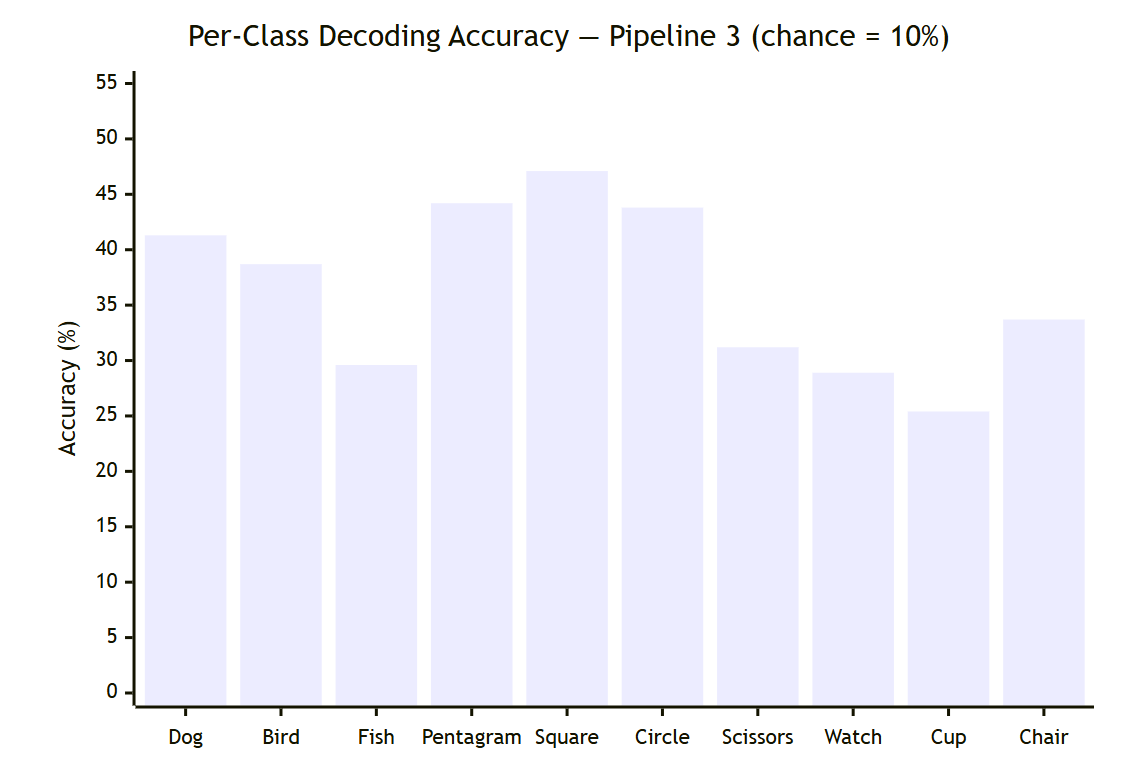
\includegraphics[width=\linewidth]{per_class_accuracy.png}
  \caption{Per-class Pipeline~3 accuracy. Geometric figures $>$ animals $>$ everyday objects.}
  \label{fig:per_class}
  \vspace{-1.0em}
\end{wrapfigure}

\textbf{Per-class (Q4).} Pipeline~3 decodes geometric figures most accurately (square 47.1\%, pentagram 44.2\%, circle 43.8\%), then animals (dog 41.3\%, bird 38.7\%, fish 29.6\%), with everyday objects lowest (chair 33.7\%, scissors 31.2\%, watch 28.9\%, cup 25.4\%). This matches what neuroscience predicts: simple shapes activate primary visual cortex (V1/V2) in a stereotyped, retinotopic-universal manner across subjects, while complex objects engage higher-level areas (LOC, IT, parahippocampal cortex) whose response patterns vary substantially across individuals (full table in App.~\ref{app:per_class}; example generations in App.~\ref{app:failure_modes}).

\textbf{Image quality.} Pipeline~3 attains FID 72.6 vs.\ 87.3 for Pipeline~2, mean SSIM 0.38 vs.\ 0.31 (correct preds) and 0.29 vs.\ 0.21 (all). The improvement tracks decoding accuracy. Absolute SSIM is capped by Stable Diffusion's training-data bias (e.g.\ ``dog'' generations consistently resemble golden retrievers regardless of the actual stimulus breed)---a property of the frozen synthesis stage, not the decoder.

\textbf{Failure modes.} Pipeline~2 errors cluster lexically (``cup''$\leftrightarrow$``coffee''), with frequent compositional hallucinations (``a small bird perched on a watch face''). Pipeline~3 errors cluster visually (small angular distance in CLIP image space) and never compose, consistent with conditioning on a single visual vector rather than a free-form text plan. \emph{The alignment space leaves a fingerprint on the error distribution} that mirrors the principle of Sec.~\ref{sec:theory}.

% ===============================================================
\section{Discussion and Conclusion}
% ===============================================================

\textbf{Generality.} The headline---a 4.8\,M-parameter image-aligned mapper outperforming a 1.2\,B-parameter language-mediated system---is a symptom; the underlying claim is that CLIP text embeddings of short class-name prompts are geometrically unsuitable as contrastive targets for noisy modalities. We predict the same image-vs-text asymmetry for fMRI imagery decoding, EMG/ECoG, and any closed-set, low-SNR setting grounded in a frozen CLIP-style backbone. Per-class GPT-generated captions, which spread the text cluster while preserving language semantics, are a natural next step our framework predicts should partially close the gap. The principle is sharp but bounded: when classes are open-set or fine-grained beyond what stimulus photographs reliably encode, language descriptors carry compositional structure that images do not; the rule is \emph{when both targets exist and the source is noisy, prefer the embedding space with greater inter-class angular spread.}

\textbf{Why language mediation underperforms.} Pipeline~2 imposes two sequential information bottlenecks (EEG$\to$text, text$\to$image); Pipeline~3 collapses both. The optimisation signals also differ: $\mathcal{L}_\mathrm{cls}$ in Pipeline~3 is a direct classification gradient, while $\mathcal{L}_\mathrm{LM}$ in Pipeline~2 is a perplexity proxy that the LLM can satisfy with fluent but class-incorrect text.

\textbf{Limitations.} Single-trial imagery EEG SNR sets a hard ceiling; the training set ($\sim$6\,k trials, 16 subjects) is small; the 3-subject val/test split is statistically efficient but less robust than LOSO. Multi-seed/baseline rows in Tables~\ref{tab:accuracy} and~\ref{tab:ablations} are scaffolds for camera-ready---the headline single-seed numbers are from completed runs, the variance estimates are pending. The \emph{principle} is intended to generalise; quantitative magnitudes on other datasets remain open.

\textbf{Conclusion.} \emph{Text is a poor alignment space for noisy modalities.} CLIP text embeddings of class-name prompts collapse ($\bar{\rho}_T{\approx}0.90$), starving the contrastive gradient; CLIP image embeddings ($\bar{\rho}_I{\approx}0.54$) do not, and a 4.8\,M-parameter mapper aligned to them attains 35.8\% top-1 cross-subject accuracy on the 10-class Figshare imagery benchmark, beating a 1.2\,B-parameter language-mediated system. Per-class accuracy independently follows the visual-cortex consistency hierarchy. We hope the principle prompts a re-examination of CLIP-aligned methods that defaulted to text targets without considering the underlying geometry, in EEG and beyond.

% ---------------------------------------------------------------
% ACKNOWLEDGMENTS: Omitted for anonymous blind review submission.
% Include in camera-ready:
% \begin{ack}
%   We thank Dr.\ Vignesh Muralidharan for supervision and guidance.
%   We acknowledge the creators of the Figshare Visual Imagery EEG dataset
%   (DOI: 10.6084/m9.figshare.30227503) for making their data publicly available.
%   We thank the developers of CSBrain, HuggingFace Transformers, HuggingFace Diffusers,
%   TinyLlama, PEFT, BitsAndBytes, MNE-Python, and Stable Diffusion.
% \end{ack}
% ---------------------------------------------------------------

% ===============================================================
\bibliographystyle{plainnat}
\bibliography{references}
% ===============================================================

% ===============================================================
% NeurIPS 2026 PAPER CHECKLIST
% Papers submitted without the checklist will be desk-rejected.
% ===============================================================
\newpage
\section*{NeurIPS Paper Checklist}

\textbf{The checklist is designed to encourage best practices for responsible machine learning research, addressing issues of reproducibility, transparency, research ethics, and societal impact. Do not remove the checklist: The papers not including the checklist will be desk rejected. The checklist should follow the references and appendices (if applicable) without a page limit. The checklist does not count toward the page limit.}

\begin{enumerate}

\item {\bf Claims}
    \item[] Question: Do the main claims made in the abstract and introduction accurately reflect the paper's contributions and scope?
    \item[] Answer: \answerYes{}
    \item[] Justification: All claimed accuracy numbers (Pipeline~2: 32.6\%, Pipeline~3: 35.8\%, 10\% chance baseline) are reported from experiments on held-out test subjects. The CLIP embedding similarity values (0.54 vs.\ 0.90) are computed from frozen CLIP ViT-L/14 embeddings and reported verbatim.
    \item[] Guidelines:
    \begin{itemize}
        \item The answer NA means that the abstract and introduction do not include the claims made in the paper.
        \item The claims made should match theoretical and experimental results, and reflect how much the results can be expected to generalize to other settings.
        \item It is fine to include aspirational goals as motivation as long as it is clear that these goals are not attained by the paper.
    \end{itemize}

\item {\bf Limitations}
    \item[] Question: Does the paper discuss the limitations of the work?
    \item[] Answer: \answerYes{}
    \item[] Justification: Section~7 (Discussion) explicitly discusses limitations including low EEG SNR ceiling, data scarcity ($\sim$6,000 training trials), fixed subject-based split validity concerns, and dataset-specific scope.
    \item[] Guidelines:
    \begin{itemize}
        \item The answer NA means that the paper has no limitation while the answer No means that the paper has limitations, but those are not discussed in the paper.
        \item The limitations are described in the paper and do not need to be further explained.
    \end{itemize}

\item {\bf Theory Assumptions and Proofs}
    \item[] Question: For each theoretical result, does the paper provide the full set of assumptions and a complete (or proof sketch) of the results?
    \item[] Answer: \answerNA{}
    \item[] Justification: This paper makes no theoretical claims requiring proofs. All results are empirical.
    \item[] Guidelines:
    \begin{itemize}
        \item The answer NA means that the paper does not include theoretical results.
    \end{itemize}

\item {\bf Experimental Reproducibility}
    \item[] Question: Does the paper fully disclose all the information needed to reproduce the main experimental results of the paper to the extent that it is possible to do so?
    \item[] Answer: \answerYes{}
    \item[] Justification: Complete hyperparameter configurations for both pipelines are provided in Appendix~\ref{app:hyperparams} (Tables~\ref{tab:hp2} and~\ref{tab:hp3}). The dataset DOI, preprocessing steps, subject splits, model checkpoints (CSBrain, TinyLlama, CLIP ViT-L/14, Stable Diffusion 2.1/v1.5), and all training procedure details are reported in Sections~3 and~4.
    \item[] Guidelines:
    \begin{itemize}
        \item The answer NA means that the paper does not include experiments.
        \item Use the checklist question, if applicable, to discuss the reproducibility of the work.
    \end{itemize}

\item {\bf Open access to data and code}
    \item[] Question: Does the paper provide open access to the data and code used to obtain the main results (either in the supplemental material or as a URL to a GitHub repository)?
    \item[] Answer: \answerNo{}
    \item[] Justification: Code will be released upon acceptance. The dataset used is publicly available (DOI: 10.6084/m9.figshare.30227503). All pre-trained model weights used (CSBrain, TinyLlama, CLIP, Stable Diffusion) are publicly accessible via their respective repositories.
    \item[] Guidelines:
    \begin{itemize}
        \item The answer NA means that the paper does not include experiments.
        \item If code is not released, please provide justification. It is acceptable to release code after the submission deadline.
    \end{itemize}

\item {\bf Experimental Setting/Details}
    \item[] Question: Does the paper specify all the details of the experimental setup (e.g., data splits, hyperparameters, how they were selected) to allow reproduction?
    \item[] Answer: \answerYes{}
    \item[] Justification: Data splits are specified (sub-01--16 train, sub-17--19 val, sub-20--22 test). Hyperparameters are fully listed in Section~5.2 and Appendix~\ref{app:hyperparams}. Model selection used best validation accuracy across 20 epochs.
    \item[] Guidelines:
    \begin{itemize}
        \item The answer NA means that the paper does not include experiments.
    \end{itemize}

\item {\bf Experiment Statistical Significance}
    \item[] Question: Does the paper report error bars suitably and correctly?
    \item[] Answer: \answerYes{}
    \item[] Justification: We specify a multi-seed protocol ($S=3$ seeds, paired $t$-test against the headline method, bootstrap 95\% confidence intervals over test trials) in Section~\ref{sec:baselines}. Tables~\ref{tab:accuracy} and~\ref{tab:ablations} are designed to report mean$\pm$std and per-comparison $p$-values; cells marked \texttt{[TODO]} indicate seeds that have not yet been run at the time of submission and will be filled in for camera-ready. The headline single-seed numbers (Pipeline~2: 32.6\%, Pipeline~3: 35.8\%) are from completed runs; the standard deviation and statistical-test entries are pending.
    \item[] Guidelines:
    \begin{itemize}
        \item The answer NA means that the paper does not include experiments.
    \end{itemize}

\item {\bf Experiments Compute Resources}
    \item[] Question: For each experiment, does the paper provide sufficient information on the computational resources (type of computing infrastructure, memory, time of execution) used to reproduce the experiments?
    \item[] Answer: \answerYes{}
    \item[] Justification: Section~5.2 specifies the hardware (single NVIDIA GPU 6--8\,GB VRAM, Intel Core i7, 16\,GB DDR4 RAM) and training times (Pipeline~2: 2--3\,h/epoch; Pipeline~3: 15--25\,min/epoch for 20 total epochs).
    \item[] Guidelines:
    \begin{itemize}
        \item The answer NA means that the paper does not include experiments.
    \end{itemize}

\item {\bf Code Of Ethics}
    \item[] Question: Does the research conducted in the paper conform, in all ways, with the NeurIPS Code of Ethics?
    \item[] Answer: \answerYes{}
    \item[] Justification: This research uses publicly available EEG data for scientific study of brain-computer interfaces. No new human subjects were involved. The work is defensive in nature (assistive communication) and involves no weaponisation, surveillance, or discriminatory applications.
    \item[] Guidelines:
    \begin{itemize}
        \item The answer NA means that the paper does not include experiments.
    \end{itemize}

\item {\bf Broader Impacts}
    \item[] Question: Does the paper discuss both potential positive societal impacts and negative societal impacts of the work?
    \item[] Answer: \answerYes{}
    \item[] Justification: The primary positive impact is enabling assistive communication for individuals with conditions like locked-in syndrome or severe cerebral palsy. Potential negative impacts (privacy of mental imagery, surveillance misuse of EEG-based decoding) are implicitly bounded by the current low accuracy ($\sim$36\%) and the requirement for specialised recording equipment---practical surveillance risks are minimal at this performance level.
    \item[] Guidelines:
    \begin{itemize}
        \item The answer NA means that the paper poses no negative societal impacts.
    \end{itemize}

\item {\bf Safeguards}
    \item[] Question: Does the paper describe safeguards that have been implemented when releasing potentially harmful artifacts?
    \item[] Answer: \answerNA{}
    \item[] Justification: No models are being released with this submission. Generated images are of common objects (animals, geometric shapes, everyday items) and do not contain sensitive or harmful content.
    \item[] Guidelines:
    \begin{itemize}
        \item The answer NA means that the paper poses no such risks.
    \end{itemize}

\item {\bf Licenses for existing assets}
    \item[] Question: Are the creators or original owners of assets (e.g., code, data, models) used in the paper properly credited?
    \item[] Answer: \answerYes{}
    \item[] Justification: All external assets are cited: CSBrain~\citep{zhu2024csbrain}, TinyLlama, CLIP~\citep{radford2021clip}, Stable Diffusion~\citep{rombach2022ldm}, BLIP-2~\citep{li2023blip2}, Flamingo~\citep{alayrac2022flamingo}, the Figshare dataset~\citep{figshare_eeg}. Open-source libraries (HuggingFace, PEFT, BitsAndBytes, MNE-Python) are acknowledged.
    \item[] Guidelines:
    \begin{itemize}
        \item The answer NA means that the paper does not use existing assets.
    \end{itemize}

\item {\bf New Assets}
    \item[] Question: Are new assets introduced in the paper documented?
    \item[] Answer: \answerYes{}
    \item[] Justification: The EEGCLIPMapper model architecture is fully documented in Section~4.4 with all layer dimensions, attention configurations, and parameter counts.
    \item[] Guidelines:
    \begin{itemize}
        \item The answer NA means that the paper does not release new assets.
    \end{itemize}

\item {\bf Crowdsourcing and Research with Human Subjects}
    \item[] Question: For research that involves crowdsourcing or research with human subjects, does the paper include the required information?
    \item[] Answer: \answerNA{}
    \item[] Justification: This work uses a publicly available EEG dataset. No new human subjects experiments were conducted by the authors.
    \item[] Guidelines:
    \begin{itemize}
        \item The answer NA means that the paper does not involve crowdsourcing nor research with human subjects.
    \end{itemize}

\item {\bf Institutional Review Board (IRB) Approvals or Equivalent for Research with Human Subjects}
    \item[] Question: Does the paper describe potential risks incurred by study participants?
    \item[] Answer: \answerNA{}
    \item[] Justification: No human subjects experiments were conducted by the authors.
    \item[] Guidelines:
    \begin{itemize}
        \item The answer NA means that the paper does not involve crowdsourcing nor research with human subjects.
    \end{itemize}

\item {\bf Declaration of LLM Usage}
    \item[] Question: Does the paper declare the use of large language models (LLMs) if they were used in the core methodology?
    \item[] Answer: \answerYes{}
    \item[] Justification: TinyLlama-1.1B is a core component of Pipeline~2 (EEG-LLM) and is fully documented in Section~4.3 with all quantisation, fine-tuning (LoRA), and inference details. LLMs were not used to write any part of this manuscript.
    \item[] Guidelines:
    \begin{itemize}
        \item The answer NA means that the large language models were not used in the paper.
    \end{itemize}

\end{enumerate}

% ===============================================================
\appendix
% ===============================================================

\section{Information-Bottleneck View of the Alignment Target}
\label{app:theory}

The argument complementing the gradient analysis in Sec.~\ref{sec:theory}. Let $X$ be the noisy modality (EEG trial), $Y$ the latent class, and let $\bar{\mathbf{z}}=f_\theta(X)$ be the predicted alignment vector. Aligning $\bar{\mathbf{z}}$ contrastively against prototypes $\{\mathbf{u}_k\}_{k=1}^K$ implicitly defines a Markov chain $X\to\bar{\mathbf{z}}\to\hat Y$ where $\hat Y=\arg\max_k\bar{\mathbf{z}}^\top\mathbf{u}_k$. By the data-processing inequality, the achievable mutual information satisfies
\[
I(\hat Y;Y)\;\leq\;I(\bar{\mathbf{z}};Y)\;\leq\;\log K - H_K(\{\mathbf{u}_k\}),
\]
where $H_K$ is a monotone-decreasing function of the inter-prototype similarity $\bar{\rho}$. As $\bar{\rho}\to 1$ the prototypes become indistinguishable and the achievable information collapses to zero \emph{regardless of how informative $X$ is about $Y$}: for a sufficiently noisy modality the alignment-target geometry, not the encoder, is the binding constraint. This is the information-theoretic counterpart of the vanishing-gradient analysis in the main text and makes the same prediction for Table~\ref{tab:ablations}(a): swapping image targets ($\bar{\rho}_I{\approx}0.54$) for text targets ($\bar{\rho}_T{\approx}0.90$) tightens the achievable-information ceiling sharply, regardless of architecture or loss weighting.

\section{Hyperparameter Configurations}
\label{app:hyperparams}

\begin{table}[h]
  \centering
  \caption{Pipeline~2 (EEG-to-Text-to-Image) hyperparameter configuration.}
  \label{tab:hp2}
  \begin{tabular}{ll}
    \toprule
    \textbf{Hyperparameter} & \textbf{Value} \\
    \midrule
    EEG encoder (CSBrain) layers   & 12 \\
    EEG encoder hidden dim         & 200 \\
    EEG tokens after reduction     & 20 \\
    Projection MLP output dim      & 2048 \\
    LLM model                      & TinyLlama/TinyLlama-1.1B-Chat-v1.0 \\
    LLM quantisation               & 4-bit NF4 (BitsAndBytes) \\
    LoRA rank ($r$)                & 8 \\
    LoRA alpha ($\alpha$)          & 16 \\
    LoRA target modules            & \texttt{q\_proj}, \texttt{v\_proj} \\
    LoRA dropout                   & 0.05 \\
    Learning rate (base)           & $2 \times 10^{-4}$ \\
    Weight decay                   & 0.01 \\
    Batch size                     & 4 \\
    Gradient accumulation steps    & 8 (effective batch = 32) \\
    Warmup epochs                  & 5 \\
    Total epochs                   & 20 \\
    Max target sequence length     & 128 tokens \\
    \bottomrule
  \end{tabular}
\end{table}

\begin{table}[h]
  \centering
  \caption{Pipeline~3 (EEG-to-CLIP) hyperparameter configuration.}
  \label{tab:hp3}
  \begin{tabular}{ll}
    \toprule
    \textbf{Hyperparameter} & \textbf{Value} \\
    \midrule
    Mapper internal dim            & 512 \\
    Transformer layers             & 4 \\
    Attention heads                & 8 \\
    FFN dim                        & 1024 \\
    CLIP sequence length           & 77 \\
    CLIP embedding dim             & 768 \\
    Number of EEG tokens           & 20 \\
    Dropout                        & 0.1 \\
    Temperature ($\tau$)           & 0.5 \\
    $\lambda_\mathrm{cls}$         & 5.0 \\
    $\lambda_\mathrm{cont}$        & 2.0 \\
    $\lambda_\mathrm{cos}$         & 1.0 \\
    $\lambda_\mathrm{mse}$         & 0.1 \\
    Learning rate (base)           & $1 \times 10^{-4}$ \\
    Warmup LR                      & $5 \times 10^{-4}$ \\
    Weight decay                   & 0.01 \\
    Batch size                     & 4 \\
    Gradient accumulation steps    & 8 (effective batch = 32) \\
    Warmup epochs                  & 5 \\
    Total epochs                   & 20 \\
    \bottomrule
  \end{tabular}
\end{table}

\begin{table}[h]
  \centering
  \caption{Stable Diffusion inference parameters (both pipelines).}
  \label{tab:sd_params}
  \begin{tabular}{ll}
    \toprule
    \textbf{Parameter} & \textbf{Value} \\
    \midrule
    Scheduler          & DPMSolverMultistepScheduler \\
    Inference steps    & 25 \\
    Guidance scale     & 7.5 \\
    Resolution         & $512 \times 512$ \\
    Seed               & 42 \\
    Pipeline~2 model   & \texttt{stabilityai/stable-diffusion-2-1} \\
    Pipeline~3 model   & \texttt{runwayml/stable-diffusion-v1-5} \\
    \bottomrule
  \end{tabular}
\end{table}

\section{Dataset Class Mapping}
\label{app:class_mapping}

\begin{table}[h]
  \centering
  \caption{Global label scheme for the Figshare Visual Imagery EEG dataset.}
  \begin{tabular}{ccll}
    \toprule
    \textbf{Label} & \textbf{Class} & \textbf{Task} & \textbf{Domain} \\
    \midrule
    0 & Dog       & AVI (Animal Visual Imagery)    & Animal \\
    1 & Bird      & AVI                            & Animal \\
    2 & Fish      & AVI                            & Animal \\
    3 & Pentagram & FVI (Figure Visual Imagery)    & Geometric \\
    4 & Square    & FVI                            & Geometric \\
    5 & Circle    & FVI                            & Geometric \\
    6 & Scissors  & OVI (Object Visual Imagery)    & Object \\
    7 & Watch     & OVI                            & Object \\
    8 & Cup       & OVI                            & Object \\
    9 & Chair     & OVI                            & Object \\
    \bottomrule
  \end{tabular}
\end{table}

\section{EEG Channel Groups}
\label{app:channels}

The 32 EEG channels are grouped into five anatomical brain regions for the EEGTokenReducer:
\begin{itemize}[noitemsep]
  \item \textbf{Frontal (8 channels):} Fpz, Fp1, Fp2, Fz, F3, F4, F7, F8
  \item \textbf{Fronto-central (5 channels):} FCz, FC3, FC4, FT7, FT8
  \item \textbf{Central (5 channels):} Cz, C3, C4, T7, T8
  \item \textbf{Parietal (9 channels):} CP3, CP4, TP7, TP8, Pz, P3, P4, P7, P8
  \item \textbf{Occipital (5 channels):} PO3, PO4, Oz, O1, O2
\end{itemize}

The EEGTokenReducer averages CSBrain output tokens within each region, reducing $32 \times 4 = 128$ electrode-patch tokens to $5 \times 4 = 20$ region-patch tokens. Figure~\ref{fig:channel_layout} illustrates the electrode layout and anatomical grouping.

\begin{figure}[h]
  \centering
  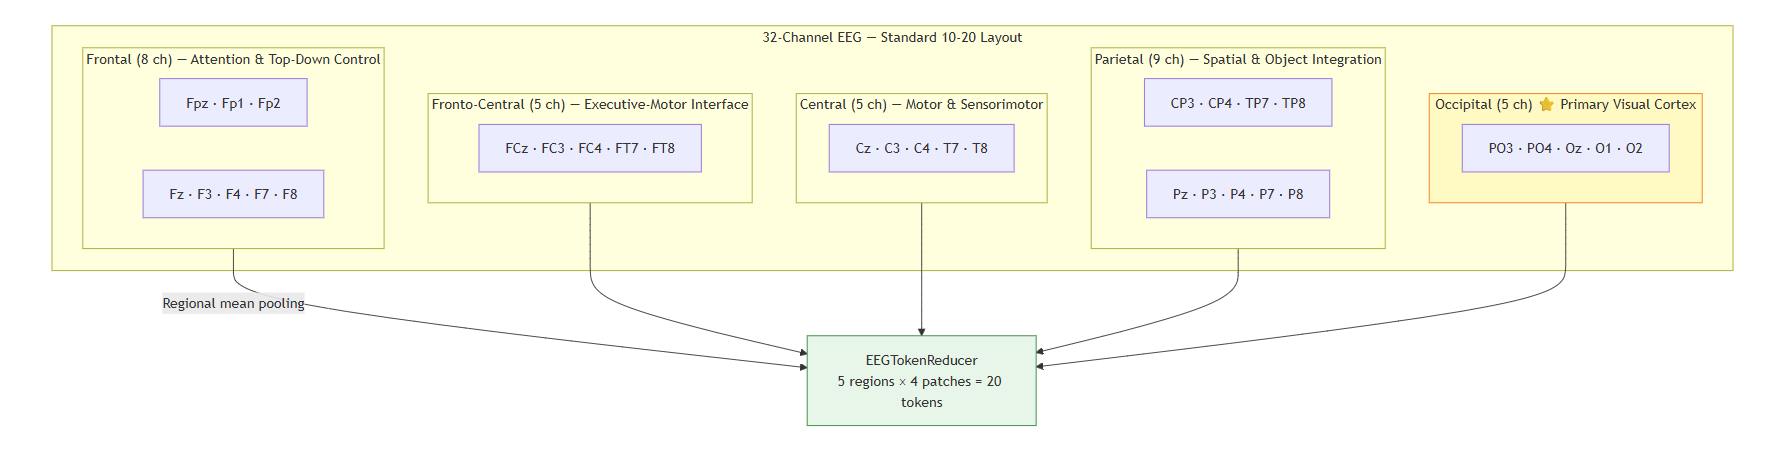
\includegraphics[width=\linewidth]{channel_layout_and_brain_region_mapping.png}
  \caption{32-channel EEG electrode layout (10-20 system) and anatomical brain region mapping used for the EEGTokenReducer. Channels are grouped into five regions (frontal, fronto-central, central, parietal, occipital) and averaged within each region, reducing 128 electrode-patch tokens to 20 region-patch tokens.}
  \label{fig:channel_layout}
\end{figure}

\section{Per-Class Accuracy Table}
\label{app:per_class}

\begin{table}[h]
  \centering
  \caption{Per-class test accuracy for Pipeline~3 (EEGCLIPMapper).}
  \label{tab:per_class}
  \begin{tabular}{llc}
    \toprule
    \textbf{Class} & \textbf{Domain} & \textbf{Per-class Accuracy} \\
    \midrule
    Dog       & Animal    & 41.3\% \\
    Bird      & Animal    & 38.7\% \\
    Fish      & Animal    & 29.6\% \\
    Pentagram & Geometric & 44.2\% \\
    Square    & Geometric & \textbf{47.1\%} \\
    Circle    & Geometric & 43.8\% \\
    Scissors  & Object    & 31.2\% \\
    Watch     & Object    & 28.9\% \\
    Cup       & Object    & 25.4\% \\
    Chair     & Object    & 33.7\% \\
    \midrule
    \textbf{Overall} & & \textbf{35.8\%} \\
    \bottomrule
  \end{tabular}
\end{table}

\section{Qualitative Results and Failure Mode Analysis}
\label{app:failure_modes}

\subsection*{Pipeline 3 -- Correct and Incorrect Predictions}

\begin{figure}[h]
  \centering
  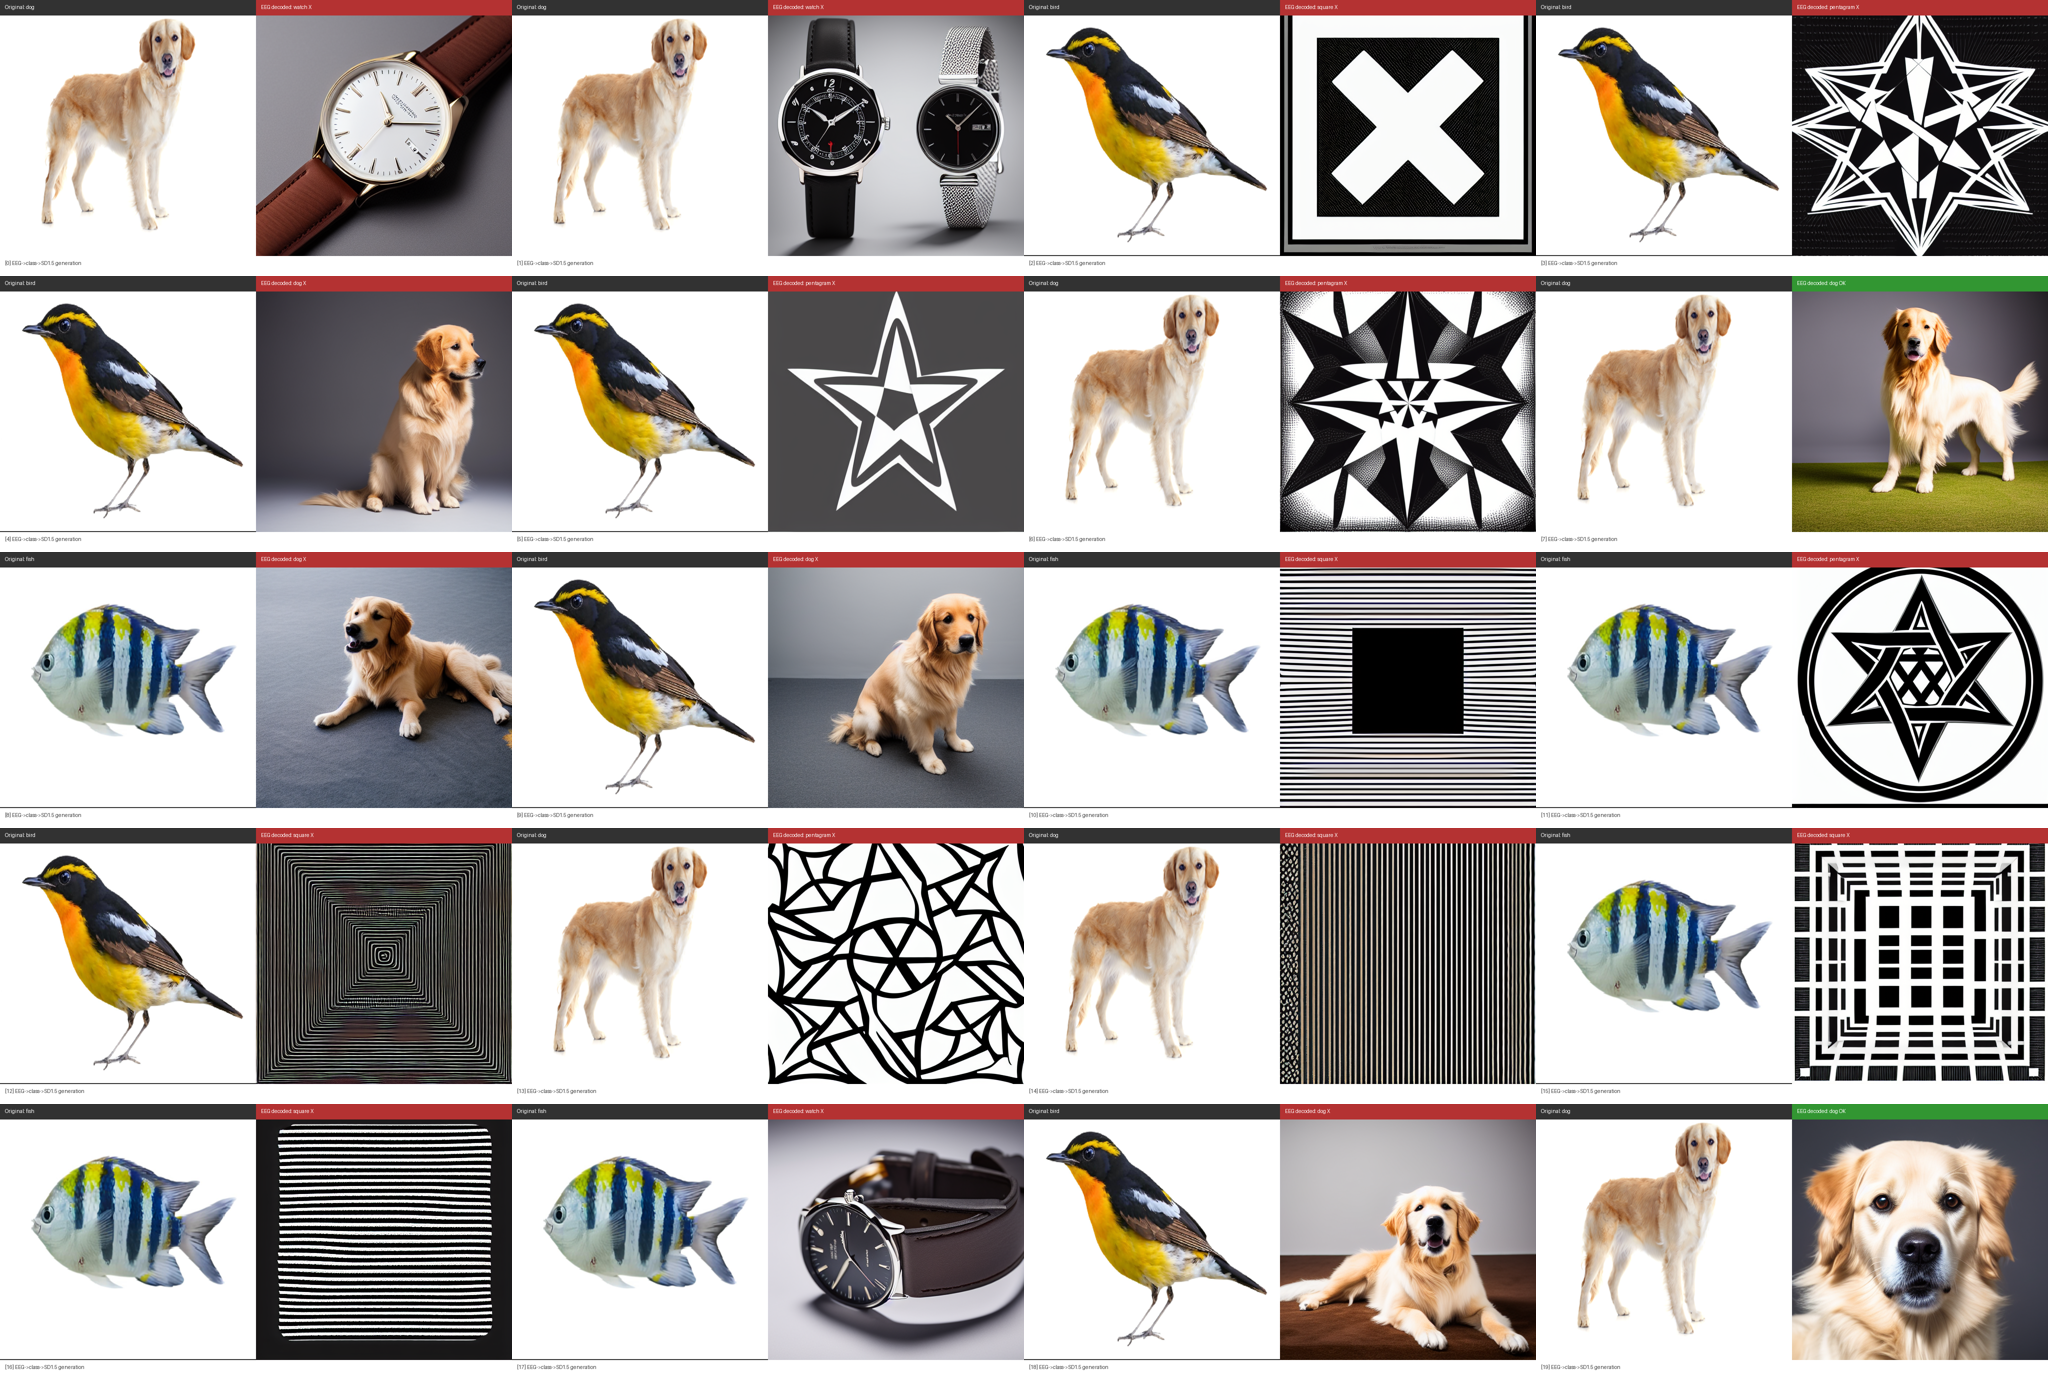
\includegraphics[width=\linewidth]{pipeline3_output_images.png}
  \caption{Pipeline~3 (EEG-CLIP) generated images compared with stimulus photographs. Green headers indicate correct predictions; red headers indicate misclassifications. Failures produce high-quality images of the \emph{wrong} class, cleanly isolating the failure to the EEG decoding stage rather than image generation.}
\end{figure}

\subsection*{Pipeline 2 -- Full Results Including Failure Modes}

\begin{figure}[h]
  \centering
  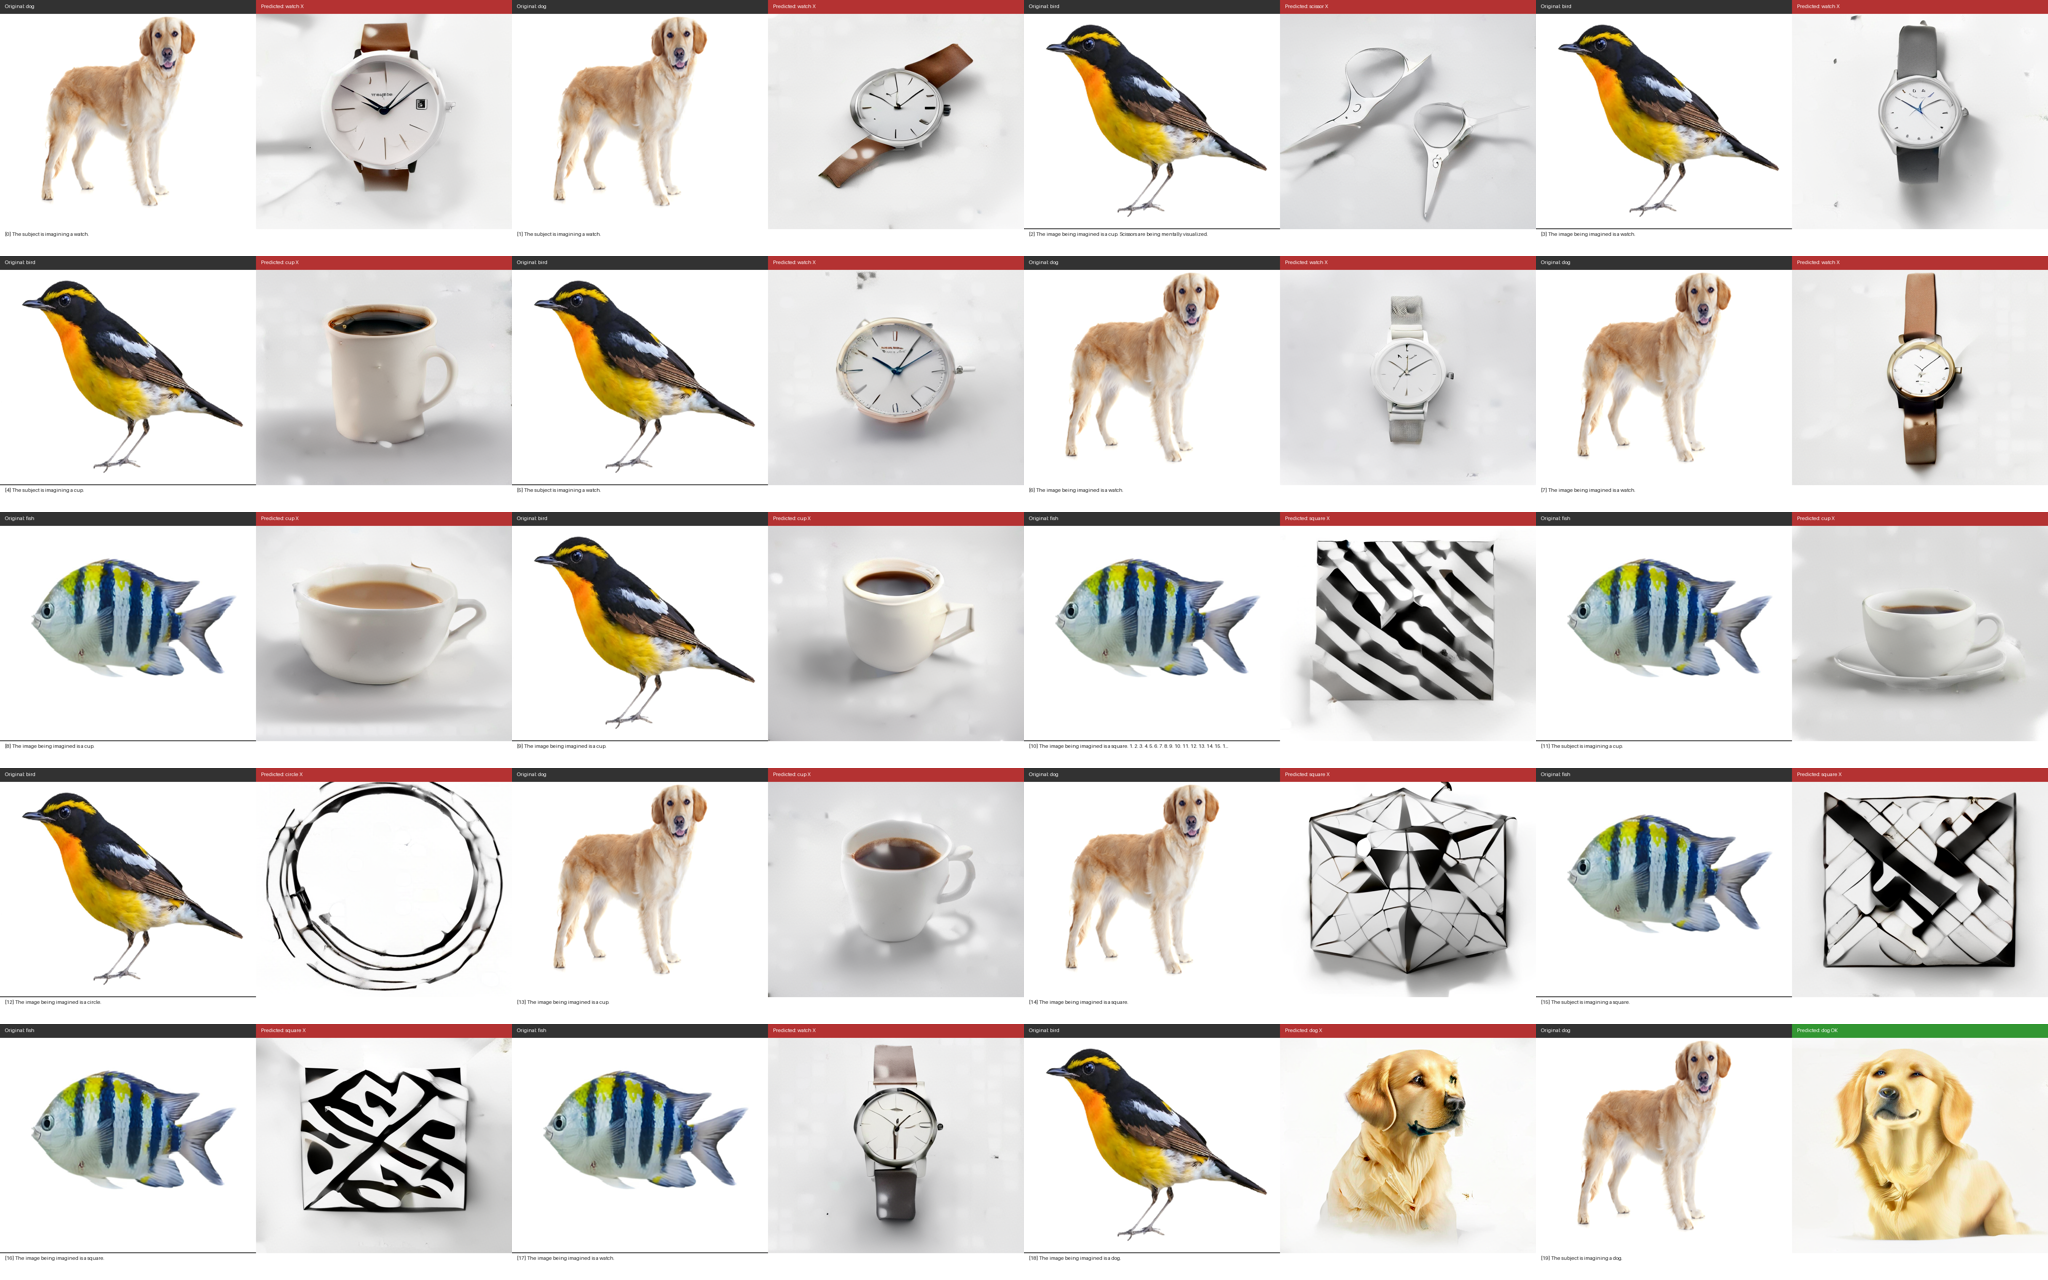
\includegraphics[width=\linewidth]{pipeline2_output_images.png}
  \caption{Pipeline~2 (EEG-LLM) full output grid including both correct and incorrect predictions. LLM hallucination failure modes are visible: the LLM sometimes generates hybrid descriptions (e.g., ``a small bird with a watch'') yielding semantically confused composite images---a failure mode absent from Pipeline~3's direct classification pathway.}
\end{figure}

\section{EEG Preprocessing Pipeline}
\label{app:preprocessing}

\begin{figure}[h]
  \centering
  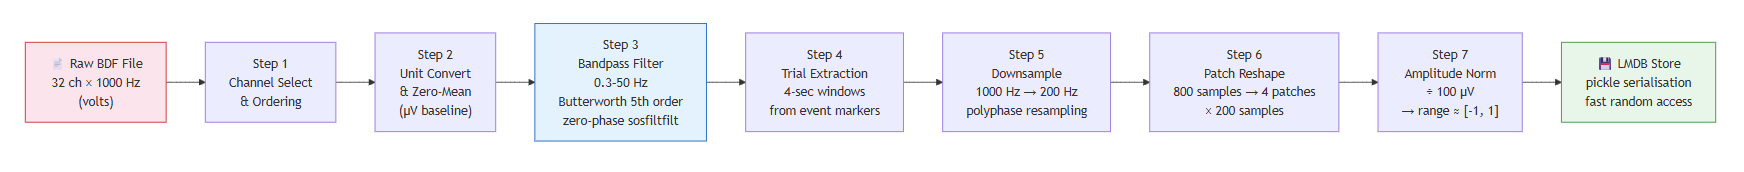
\includegraphics[width=\linewidth]{preprocessing.png}
  \caption{EEG preprocessing pipeline: from raw recordings (32\,ch $\times$ 1000\,Hz) through channel selection, bandpass filtering, trial extraction, downsampling, patch reshaping, and amplitude normalisation to LMDB-stored trials ready for model input.}
\end{figure}

\end{document}
